\chapter{Gradient Descent}

\begin{goals}
\begin{itemize}
    \item Review calculus: derivatives measure sensitivity
    \item Understand gradient descent as iterative optimization
    \item See Newton's method and its quadratic convergence
    \item Appreciate why continuous optimization is powerful
\end{itemize}
\end{goals}

\section{The Optimization Problem}

We have a function $f : \mathbb{R}^n \to \mathbb{R}$ and want to find:
\[
\theta^* = \arg\min_\theta f(\theta)
\]

If $f$ is differentiable, the gradient $\nabla f(\theta)$ points ``uphill.''

\begin{intuition}
The gradient tells you: ``If you want $f$ to increase, go this direction.'' So to minimize, go the opposite direction.
\end{intuition}

\section{Gradient Descent}

\begin{definition}[Gradient Descent]
Starting from $\theta_0$, iterate:
\[
\theta_{t+1} = \theta_t - \eta \nabla f(\theta_t)
\]
where $\eta > 0$ is the \emph{learning rate}.
\end{definition}

\begin{center}
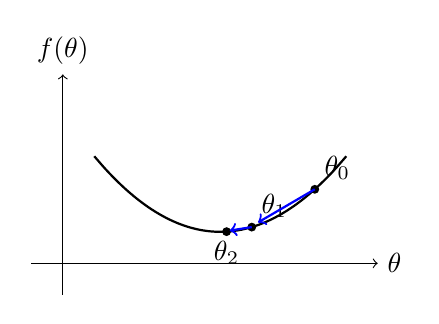
\begin{tikzpicture}[scale=0.8]
\draw[->] (-0.5,0) -- (5,0) node[right] {$\theta$};
\draw[->] (0,-0.5) -- (0,3) node[above] {$f(\theta)$};
\draw[thick, domain=0.5:4.5, smooth] plot (\x, {0.3*(\x-2.5)*(\x-2.5) + 0.5});
\fill (4,1.175) circle (2pt) node[above right] {$\theta_0$};
\fill (3,0.575) circle (2pt) node[above right] {$\theta_1$};
\fill (2.6,0.503) circle (2pt) node[below] {$\theta_2$};
\draw[->, thick, blue] (4,1.175) -- (3.1,0.65);
\draw[->, thick, blue] (3,0.575) -- (2.65,0.52);
\end{tikzpicture}
\end{center}

\section{Convergence}

\begin{theorem}[Convergence for Convex Functions]
If $f$ is convex and $L$-smooth (bounded second derivatives), gradient descent with $\eta = 1/L$ satisfies:
\[
f(\theta_t) - f(\theta^*) \leq \frac{\|\theta_0 - \theta^*\|^2}{2t/L}
\]
\end{theorem}

Rate: $O(1/t)$. Slow, but guaranteed.

\section{Newton's Method}

Use second-order information (the Hessian $H = \nabla^2 f$):
\[
\theta_{t+1} = \theta_t - H(\theta_t)^{-1} \nabla f(\theta_t)
\]

\begin{theorem}[Quadratic Convergence]
Near a minimum with positive definite Hessian, Newton's method converges quadratically:
\[
\|\theta_{t+1} - \theta^*\| \leq C \|\theta_t - \theta^*\|^2
\]
\end{theorem}

\begin{keyinsight}
Newton's method uses curvature information to take better steps. The Hessian ``rescales'' the gradient to account for how steep different directions are.
\end{keyinsight}

\section{The Problem with Discrete Spaces}

All of this requires:
\begin{itemize}
    \item A continuous space $\mathbb{R}^n$
    \item A differentiable function $f$
\end{itemize}

But the structures we care about (automata, Kripke frames, programs) are \emph{discrete}.

\begin{warning}
You can't take the gradient of ``number of states'' or ``which transitions exist.'' Discrete spaces have no derivatives.
\end{warning}

\textbf{Solution}: Embed discrete structures into continuous spaces. This is the motivation for \emph{semirings}.
